\documentclass[conference]{IEEEtran}
\usepackage{settings}

\begin{document}

\maketitle

\begin{abstract}
We present a deep learning framework for non-invasive respiratory phase classification (inhalation/exhalation) from one-second audio clips. Our hybrid-feature approach uses nine spectral representations, including Mel-spectrograms and MFCCs, and 39 scalar features to train two distinct Convolutional Neural Networks (CNNs): a lightweight 2.43M parameter model and a larger 8.15M parameter VGG-inspired architecture. To improve generalization against real-world acoustic variability, the models are trained with CutMix and MixUp data augmentation. A final weighted ensemble of these models, with weights determined by validation performance, achieves a classification accuracy of 76.7\% on the private test set.
\end{abstract}

\section{Introduction}

\subsection{Problem Definition}

While breathing patterns offer valuable clues for detecting chronic disease, practical tools for home monitoring are missing. The existing options are simply not viable for widespread use. Hospital-grade devices are prohibitively expensive and complex, and manually reviewing audio data is an unscalable process unsuitable for real-time applications \cite{lee2025co2sensor}.

The most obvious alternative---listening to the breath---is simple and non-invasive. But it has a critical flaw. Inhales and exhales often sound remarkably alike, a similarity that confounds simple algorithms (Fig. \ref{fig:sample_waveform}). This problem is amplified by real-world conditions like background noise or differences between individuals, causing conventional acoustic methods to fail. A more sophisticated interpretive model is therefore necessary to reliably classify respiratory phases from sound alone \cite{lee2023wheezing}.

\begin{figure}[h!]
    \centering
    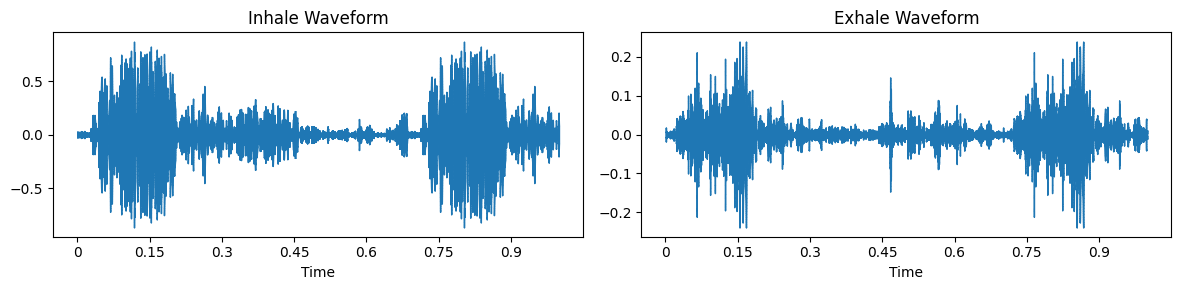
\includegraphics[width=\columnwidth]{figures/sample_waveform}	
    \caption{Example waveforms showing inhale vs exhale patterns}
    \label{fig:sample_waveform}
\end{figure}

\subsection{Research Objectives}

This study confronts the problem by designing a deep learning model specifically trained to differentiate between the subtle acoustic signatures of inhalation and exhalation. We feed a rich tapestry of acoustic information---spanning multiple spectrogram formats, frequency-domain vectors, and signal energy characteristics---into a multi-input Convolutional Neural Network(CNN).

\subsection{Dataset Overview}

The dataset provided for this study consists of 5,000 individual audio recordings of human respiratory sounds. The data is pre-partitioned into a training set of 4,000 samples and a test set of 1,000 samples. Each sample is a one-second, mono-channel audio file in the .wav format, and labled either an inhalation or an exhalation for the training set.


\section{Method}

This section details the feature extraction process, model architectures, and training procedures used for respiratory phase classification. The overall feature extraction pipeline is illustrated in Fig.~\ref{fig:feat_ext_diagram}.


\begin{figure}[h!]
\centering
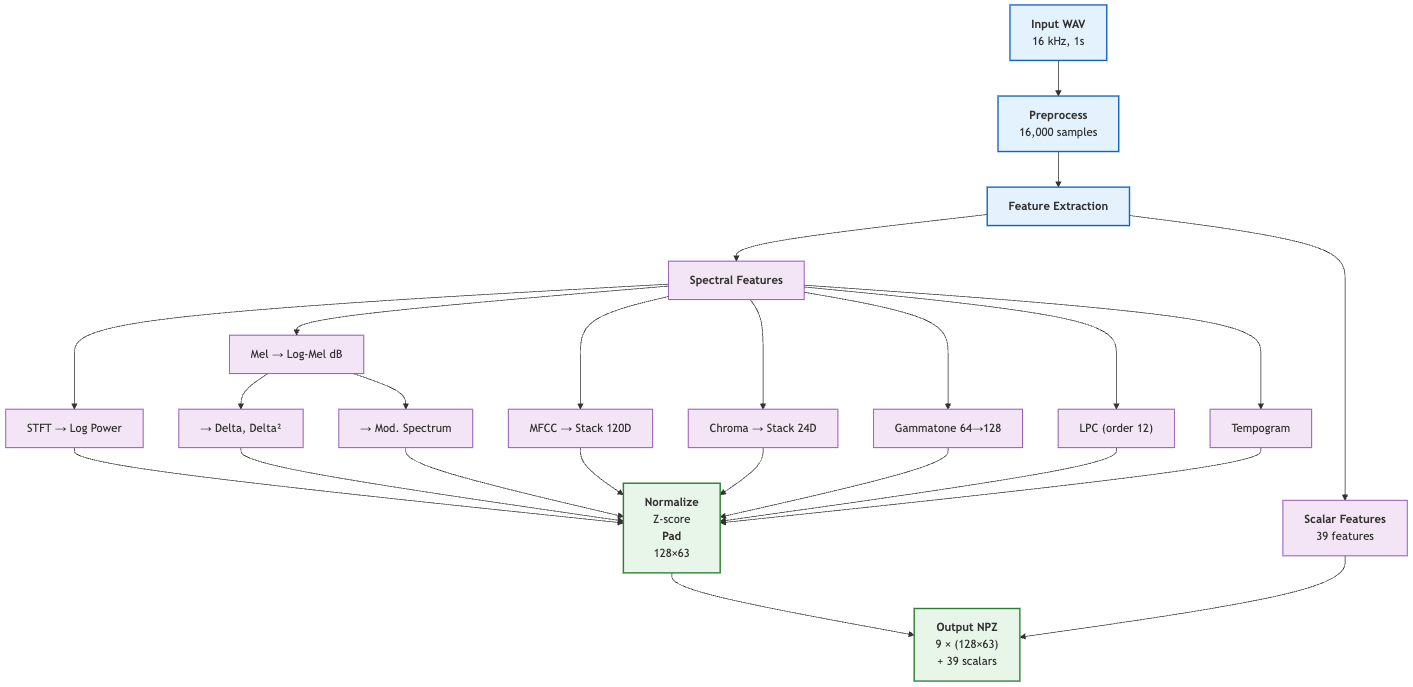
\includegraphics[width=\columnwidth]{figures/feature_extraction}	
\caption{Feature extraction pipeline diagram}
\label{fig:feat_ext_diagram}
\end{figure}

\subsection{Feature Extraction}

The input to our system is a one-second audio clip sampled at 16 kHz. From each clip, we extracted two categories of features: spectral representations and scalar values. All features were pre-computed and stored as NumPy archives to accelerate the training pipeline.

\subsubsection{Spectral Representations}

We computed nine distinct time-frequency representations: STFT, Mel-spectrogram with its first (delta) and second (delta-delta) derivatives, Mel-Frequency Cepstral Coefficients (MFCC), chroma, gammatone, modulation spectrum, and tempogram. Visual comparisons for these features are provided in Figs.~\ref{fig:stft}-\ref{fig:tempogram}. All spectral features were reshaped or padded to a uniform dimension of 128 frequency bins by 63 time steps and were normalized using z-scoring.

\begin{figure}[h!]
\centering
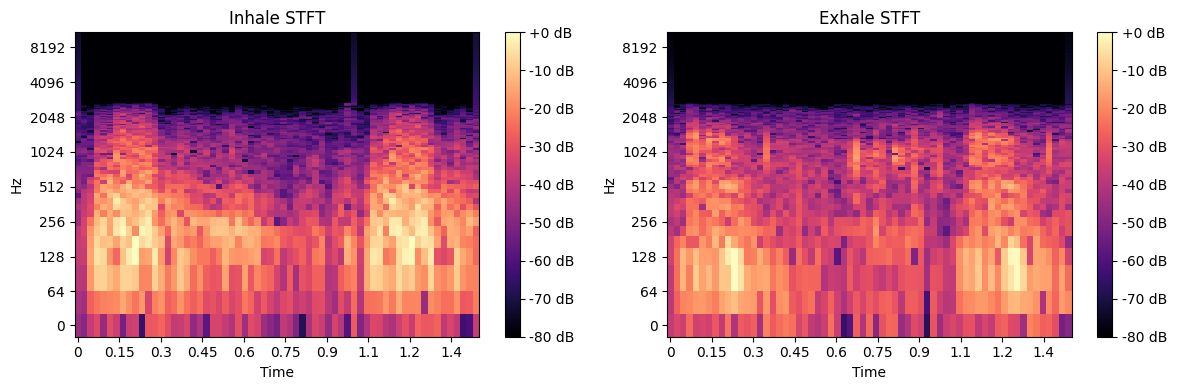
\includegraphics[width=\columnwidth]{figures/stft}	
\caption{STFT spectrograms for inhale/exhale}
\label{fig:stft}
\end{figure}

\begin{figure}[h!]
\centering
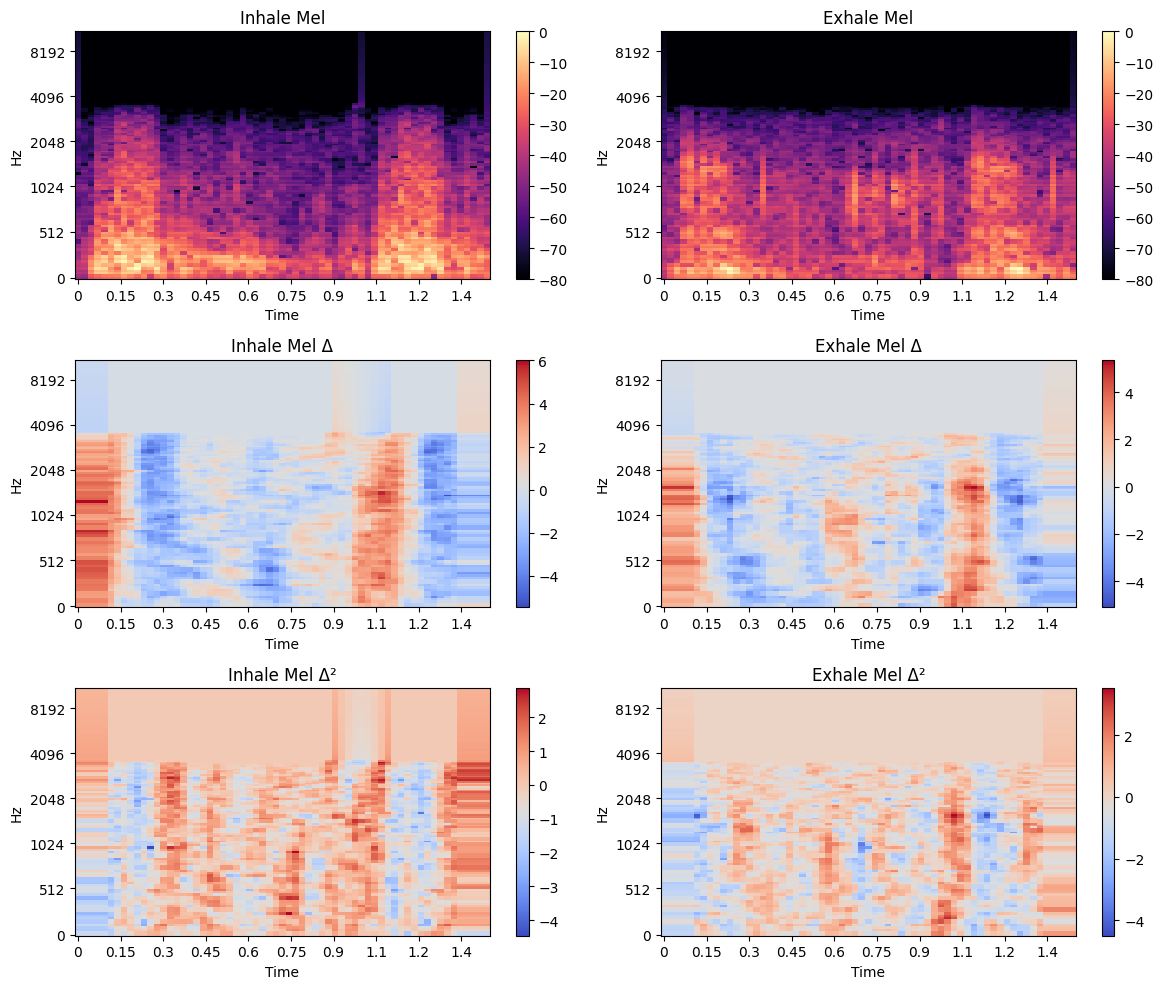
\includegraphics[width=\columnwidth]{figures/mel}	
\caption{Mel spectrograms with delta coefficients}
\label{fig:mel}
\end{figure}

\begin{figure}[h!]
\centering
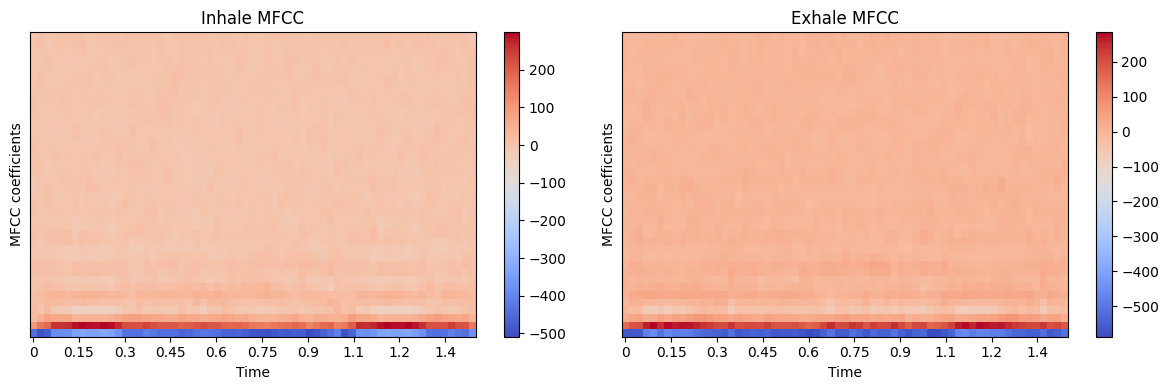
\includegraphics[width=\columnwidth]{figures/mfcc}	
\caption{MFCC comparison}
\label{fig:mfcc}
\end{figure}

\begin{figure}[ht!]
\centering
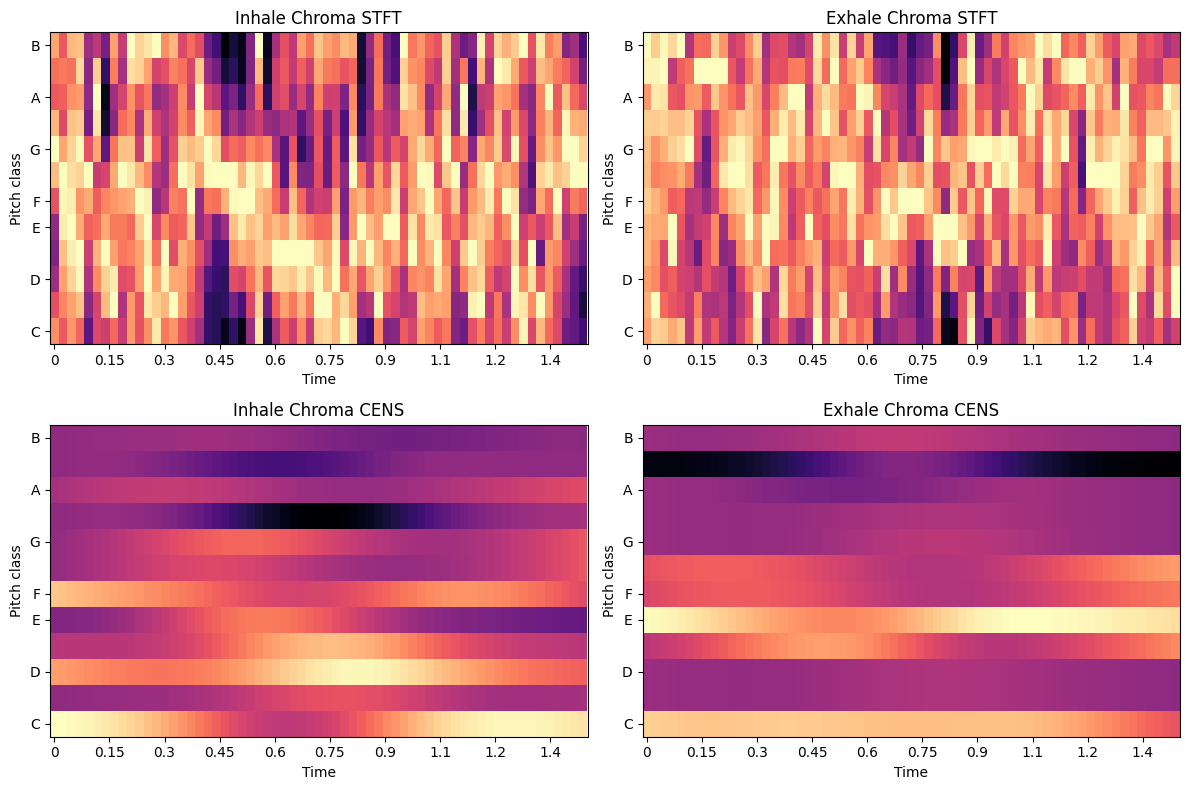
\includegraphics[width=\columnwidth]{figures/chroma}	
\caption{Chroma STFT and CENS features}
\label{fig:chroma}
\end{figure}

\begin{figure}[h!]
\centering
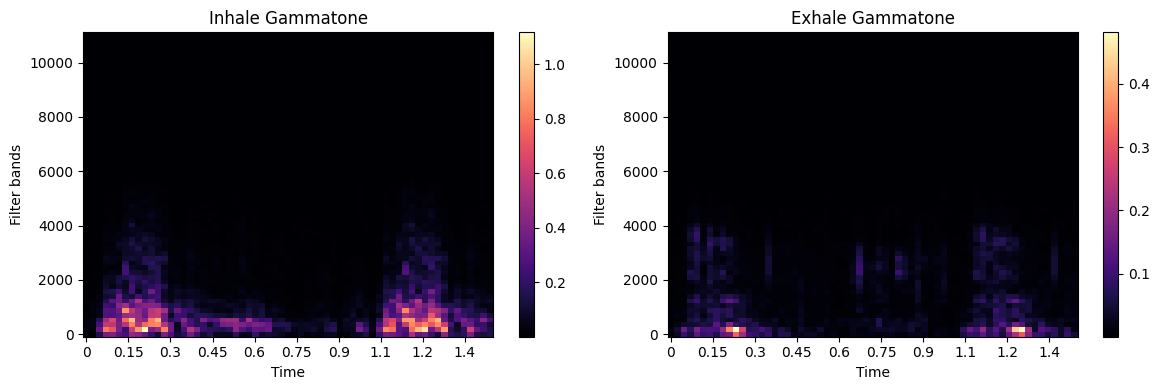
\includegraphics[width=\columnwidth]{figures/gammatone}	
\caption{Gammatone filterbank features}
\label{fig:gammatone}
\end{figure}

\begin{figure}[h!]
\centering
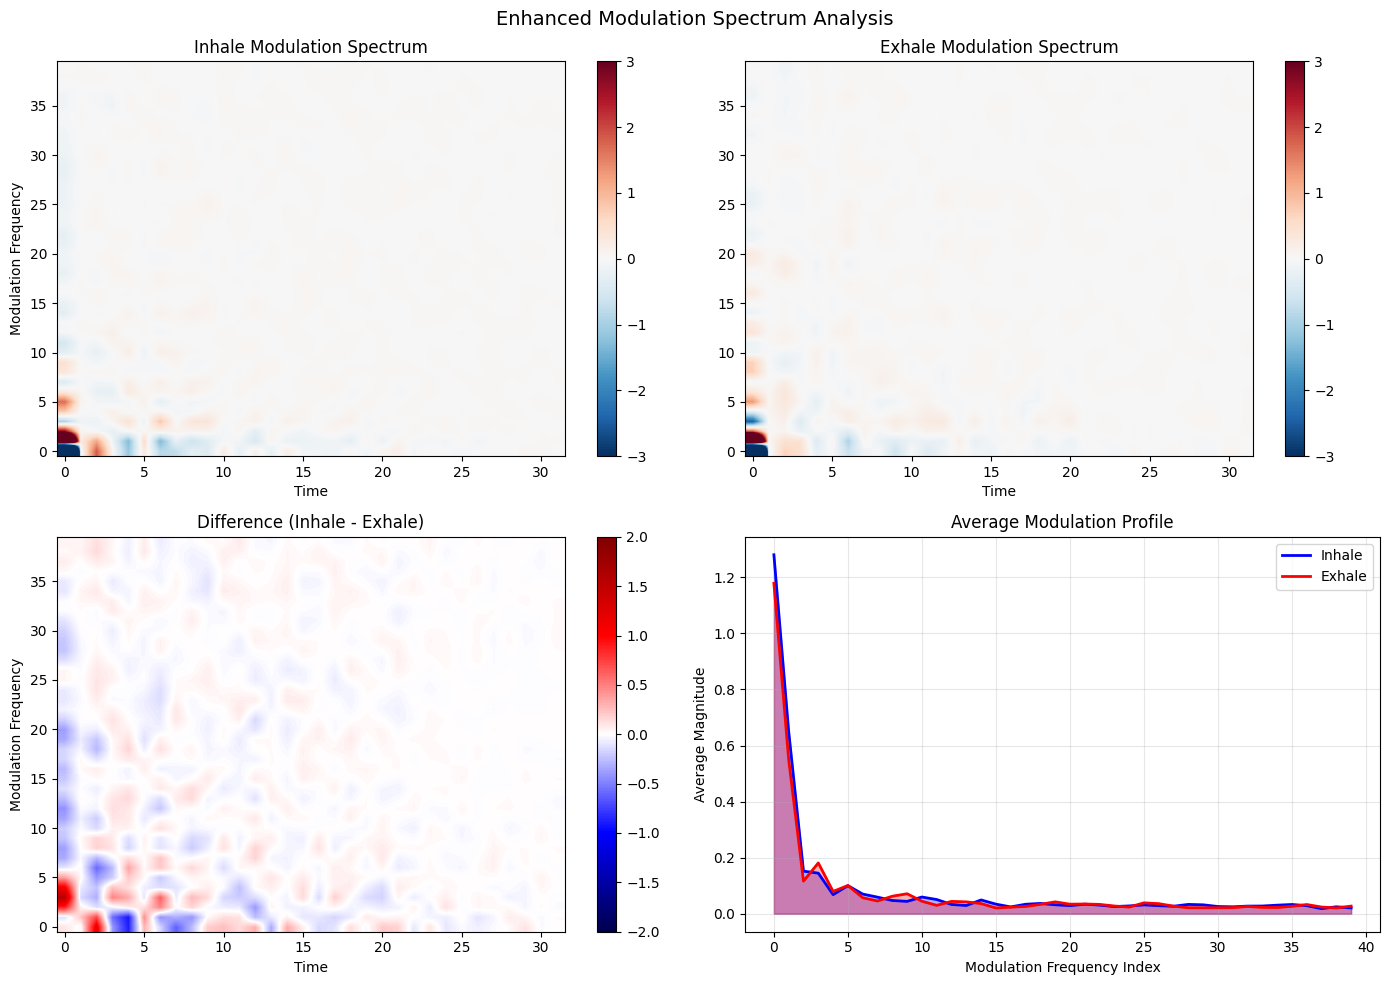
\includegraphics[width=\columnwidth]{figures/modulation}	
\caption{Modulation spectrum analysis}
\label{fig:modulation}
\end{figure}

\begin{figure}[h!]
\centering
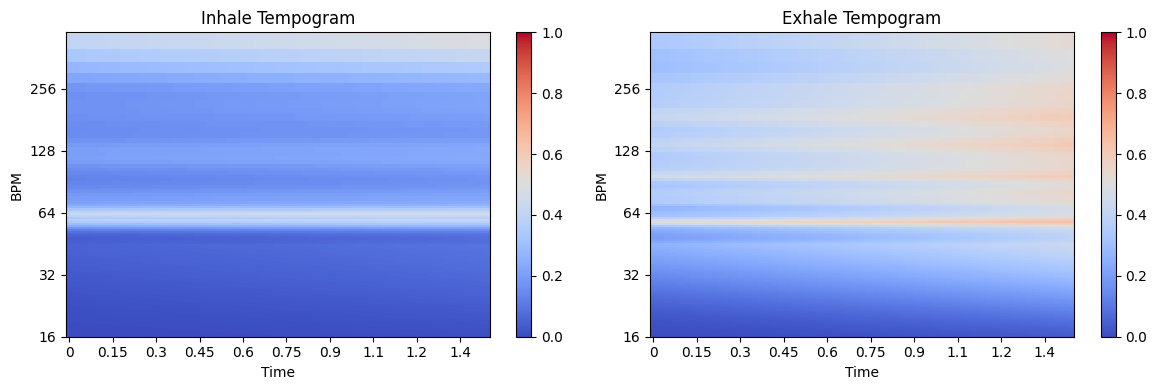
\includegraphics[width=\columnwidth]{figures/tempogram}	
\caption{Tempogram comparison}
\label{fig:tempogram}
\end{figure}

\subsubsection{Scalar Features}

We extracted 39 scalar features---spanning temporal metrics (e.g., RMS energy, ZCR) and spectral statistics (e.g., centroid, bandwidth)---to characterize the signal. Key feature comparisons between respiratory phases are plotted in Fig.~\ref{fig:scalars}.

\begin{figure}[h!]
\centering
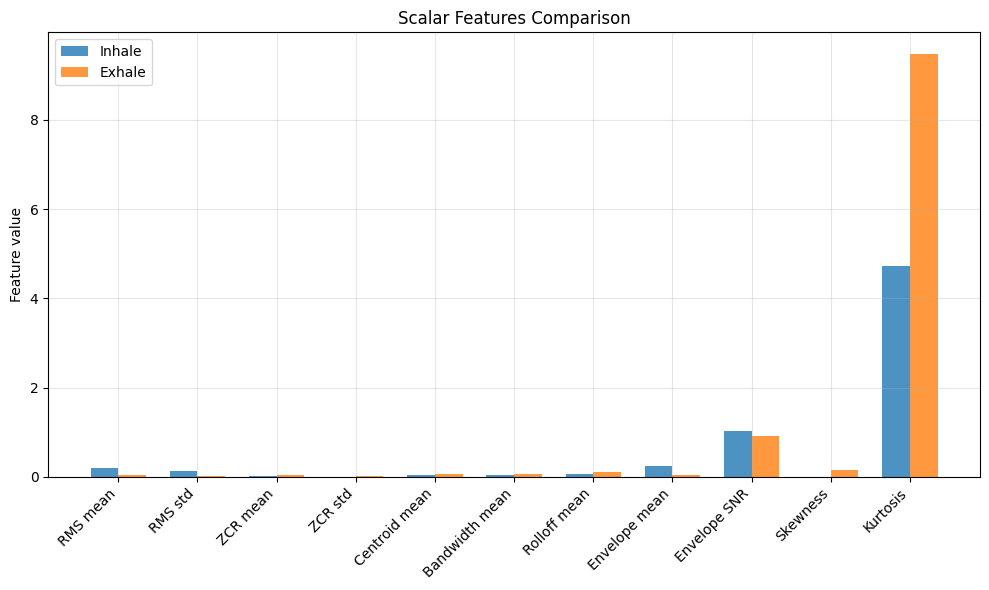
\includegraphics[width=0.9\columnwidth]{figures/scalars}	
\caption{Scalar features comparison}
\label{fig:scalars}
\end{figure}

\subsection{Model Architectures}

We designed two Convolutional Neural Network (CNN) architectures to process the combined feature sets. Each model contains a convolutional pathway for spectral features and a Multi-Layer Perceptron (MLP) pathway for scalar features.

\subsubsection{CNN8}

This is a lightweight model with eight convolutional layers organized in four blocks ($32\rightarrow64\rightarrow128\rightarrow256$ channels). It uses ReLU activations, Batch Normalization, and max pooling. The scalar pathway is a two-layer MLP.

\subsubsection{VGG-Inspired Model}

This higher-capacity model contains 12 convolutional layers in four blocks ($64\rightarrow128\rightarrow256\rightarrow512$ channels) with GELU activations. A residual connection is included in the final block. The model contains 8.15M trainable parameters.

\subsection{Training and Optimization}

\subsubsection{Optimizer}

Models were trained with the \textit{AdamW} optimizer using a weight decay, $\lambda$ of $10^{-4}$ . The learning rate followed a cosine annealing schedule with a linear warmup. Initial learning rates were set to $4\times10^{-4}$ for CNN8 and $1\times10^{-3}$ for the VGG-inspired model. Gradient norms were clipped at a maximum value of $1.0$.

\subsubsection{Data Augmentation}

After a four-epoch warmup, we applied stochastic data augmentation. The methods used were \textit{CutMix}, with a probability of 0.6, and \textit{MixUp}, with a probability of 0.4.

\subsubsection{Training Configuration}

We used a binary cross-entropy with logits loss function. The data was split into training (80\%) and validation (20\%) sets using a stratified method. Training ran for a maximum of 140 epochs with early stopping based on validation accuracy. Mixed-precision training was used to reduce computation time.

\subsection{Ensemble Method}

Final predictions for the test set were generated by an ensemble of the trained models. The sigmoid outputs of the models were combined using a weighted average, as shown in (1).

$$P_{\text{final}} = \sum_{i=1}^{N} \alpha_i \cdot \sigma(\text{logits}_i) \eqno{(1)}$$

The weights, $\alpha_i$ , were derived from the softmax-normalized validation accuracy of each contributing model, giving greater influence to better-performing models.


\section{Results}

\subsection{Model Performance}

Table~\ref{tab:performance_metrics} summarizes the performance of our two base classifiers (CNN8 and VGG-inspired) alongside their final ensemble. Although the individual models reached 77.8\% and 79.2\% accuracy on the validation split, the ensemble delivered superior real-world results---achieving 78.6\% on the Kaggle public test and 76.7\% on the private holdout---outperforming the best single model by over two percentage points and demonstrating the clear benefit of combining their complementary strengths.

\begin{table}[h!]
\centering
\caption{Comparative performance of the baseline CNN8, VGG-inspired model, and their final ensemble.}
\label{tab:performance_metrics}
\resizebox{\columnwidth}{!}{
  \begin{tabular}{@{}lccccc|cc@{}}
    \toprule
      \multirow{2}{*}{\textbf{Model}}
      & \multicolumn{5}{c|}{\textbf{Validation}} 
      & \multicolumn{2}{c}{\textbf{Test (Acc.)}} \\
    \cmidrule(lr){2-6}\cmidrule(l){7-8}
      & Acc. & AUC & Prec. & Rec. & F1 
      & Public & Private \\
    \midrule
    CNN8 & 0.778 & 0.831 & 0.780 & 0.775 & 0.777  & 0.761 & 0.737  \\
    VGG-inspired   & 0.792 & 0.845 & 0.796 & 0.789 & 0.792 & 0.771 & 0.747 \\
    \midrule
    Ensemble &   --   &  --   &   --   &   --   &   --   & \textbf{0.786} & \textbf{0.767} \\
    \bottomrule
  \end{tabular}
}
\end{table}

Also, data augmentation with CutMix and MixUp boosted our test‐set accuracy from 72.0\% (public) and 69.3\% (private) to 78.6\% and 76.7\%, respectively---an improvement of over two percentage points versus the best individual model (Fig.~\ref{fig:augmentation_result}).

\begin{figure}[h!]
  \centering
  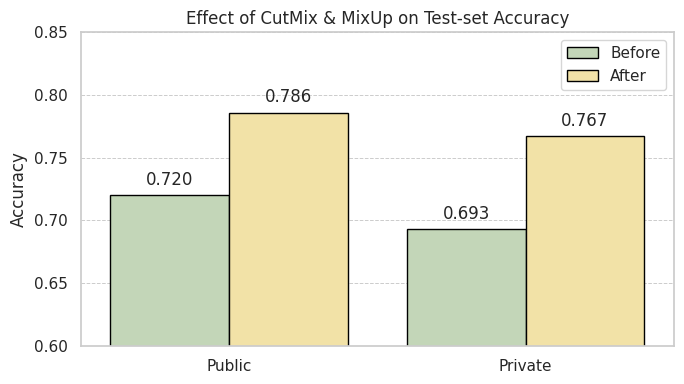
\includegraphics[width=\columnwidth]{figures/augmentation_result}
  \caption{Impact of CutMix and MixUp augmentation on Kaggle test‐set accuracy. “Before” refers to the baseline (72.0\% public / 69.3\% private); “After” shows the augmented results (78.6\% public / 76.7 \% private).}
  \label{fig:augmentation_result}
\end{figure}

\section{Discussion}

\subsection{Interpretation of Results}

A key observation from our experiments is how well data augmentation methods from computer vision, specifically CutMix and MixUp, transferred to the domain of audio spectrograms. Their success here suggests a degree of cross-domain applicability, though our results also show the model benefits from a few warmup epochs to grasp basic patterns before augmentation begins. The value of the hybrid-feature design was also clear; adding the scalar feature vector consistently improved accuracy, pointing to complementary acoustic information that spectral images alone do not capture.

One of the main takeaways is the trade-off between model size and performance. The VGG-inspired network, despite having over three times the parameters, was only marginally better than the lightweight CNN8. The fact that our ensemble outperformed both models underscores that, for this problem, combining architecturally different models is a more effective strategy than simply increasing the scale of a single network.

\subsection{Limitations}

This study has two main limitations. First, the fixed one-second segmentation of audio clips prevents the models from learning temporal dependencies that span multiple respiratory cycles. Information about the overall breathing rhythm is lost. Second, our feature engineering strategy, while effective, is fixed. An end-to-end approach that learns features directly from raw audio might discover more optimal, task-specific representations.

\subsection{Future Work}

Based on these findings, future research could proceed in several directions. To address the limitation of fixed-length inputs, recurrent or attention-based architectures (e.g., LSTMs, Transformers) could be employed to model long-range temporal context. An end-to-end learning framework should also be investigated as a potential alternative to hand-crafted features.

For clinical applicability, two extensions are proposed. First, model interpretability methods, such as gradient-based attribution, could be used to visualize which parts of a sound are most indicative of inhalation or exhalation. Second, the binary classification task could be expanded to a multi-class problem that includes other respiratory events, such as breath-holds and coughs, to create a more comprehensive monitoring tool.


\section{Conclusion}

We presented a lightweight reproducible pipeline for noninvasive detection of breathing phases from short audio clips. We extracted spectral and scalar features and used CutMix and MixUp to improve Kaggle test set accuracy from 72.0\% public and 69.3\% private to 78.6\% and 76.7\% respectively. A simple ensemble of CNN8 and a VGG inspired network added two percentage points and showed the value of model combination. The system requires no specialized hardware or manual review and suits real time home use scenarios. Future work will address classification of pathological sounds such as wheeze and evaluate end to end deep models on raw audio data to improve performance.


\appendices
\section{Code Availability}
The source code for this project is publicly available at:  \url{https://github.com/dohyeoplim/breathing-phase-classifier}

\bibliography{references.bib}

\end{document}